We evaluate the performance of B2B throughout a series of experiments on
controlled synthetic data.
%
The purpose of these experiments is to evaluate the ability of B2B in terms of
prediction of independent and identically distributed data, as well as a method
to recover causal factors.

The data generating process for each experiment constructs $n=1000$ training examples
according to the model $Y = (\text{snr} \cdot XE + N)F$, where $\text{snr}$ is a
scalar that modulates the signal-to-noise ratio.
%
Here,
%\begin{itemize} \item $F \in \mathbb{R}^{d_x \times d_y}$ contains entries
%drawn from $\mathcal{N}(0, d_x^{-1})$, \item $X \in \mathbb{R}^{n \times d_x}$
%contains rows drawn from $\mathcal{N}(0, \Sigma_X)$, \item $N \in \mathbb{R}^{n
%\times d_x}$ contains rows drawn from $\mathcal{N}(0, \Sigma_N)$, \item $E \in
%\mathbb{R}^{d_x \times d_x}$ is a binary diagonal matrix containing $n_c$ ones,
%\item $\Sigma_X = AA^\top$, where $A \in \mathbb{R}^{d_x \times d_x}$ contains
%entries drawn from $\mathcal{N}(0, d_x^{-1})$, \item $\Sigma_N = BB^\top$,
%where $B \in \mathbb{R}^{d_x \times d_x}$ contains entries drawn from
%$\mathcal{N}(0, d_x^{-1})$, \end{itemize}
    $F \in \mathbb{R}^{d_x \times d_y}$ contains entries drawn from
$\mathcal{N}(0, d_x^{-1})$, $X \in \mathbb{R}^{n \times d_x}$ contains rows
drawn from $\mathcal{N}(0, \Sigma_X)$, $N \in \mathbb{R}^{n \times d_x}$
contains rows drawn from $\mathcal{N}(0, \Sigma_N)$, $E \in \mathbb{R}^{d_x
\times d_x}$ is a binary diagonal matrix containing $n_c$ ones, $\Sigma_X =
AA^\top$ where $A \in \mathbb{R}^{d_x \times d_x}$ contains entries drawn from
$\mathcal{N}(0, d_x^{-1})$, $\Sigma_N = BB^\top$ where $B \in \mathbb{R}^{d_x
\times d_x}$ contains entries drawn from $\mathcal{N}(0, d_x^{-1})$, and the
factor $\text{snr} \in (0, \infty)$.

To simulate a wide range of experimental conditions, we sample 10 values in log-space for $d_x, d_y \in \left[ 10, 100 \right]$, $n_c \in \left[ 3, 63 \right]$,
$\text{snr} \in \left[ 0.001, 10 \right]$. We discard the cases where $n_c > d_x$, limit $d_x, d_y$ to 100 to keep the running time under 2 hours for each condition, and average over 5 random seeds.
%
% Each condition is simulated under $5$ different random seeds.

We compare the performance of B2B against four competing methods, all
implemented in scikit-learn \citep{scikit}:
%
% To be updated

\subsection{Baseline models}

Forward regression consists of an $l2$-regularized "ridge" regression from the
putative causes $X$ to the observations $Y$: \begin{equation} H = (X^T X
+\lambda I)^{-1} X^T Y \end{equation}

Backward regression consists of an $l2$-regularized "ridge" regression from $Y$
to $X$: \begin{equation} G = (Y^T Y +\lambda I)^{-1} Y^T X \end{equation}

CCA finds $G\in\mathbb{R}^{d_z, d_y}$ and $H\in\mathbb{R}^{d_z, d_x}$
% such that
s.t.
$X$ and $Y$ are maximally correlated in a latent $Z$ space:
% \begin{equation} maxcorr(XH^T, YG^T) \end{equation}
\begin{equation} G,H = \argmax_{G,H} corr(XH^T, YG^T) \end{equation}

% To be checked
PLS finds $G\in\mathbb{R}^{d_z, d_y}$ and $H\in\mathbb{R}^{d_z, d_x}$
% such that
s.t.
$X$ and $Y$ are maximally covarying in a latent $Z$ space:
% \begin{equation} maxcov(XH^T, YG^T) \end{equation}
\begin{equation} G,H = \argmax_{G,H} cov(XH^T, YG^T) \end{equation}

We employ $5$-fold cross-validation to select the optimal number of components
for CCA and PLS. Regressions were $\ell2$-regularized with a $\lambda$ regularization
parameters fitted with the efficient leave-one-out procedure implemented in
scikit-learn RidgeCV \citep{scikit}.

\subsection{Evaluating Causal Discovery from models' coefficients}

B2B leads to unbiased (i.e. zeros-centered) scalar coefficients for non-causal
features. In contrast, the Forward, Backward, CCA and PLS models lead to a
loading vector $H_i$ per feature $i$ (or one vector $G^i$ for the backward
model). To transform such vector into an estimated causal contribution $\hat E$,
we take the sum of square coefficients:
% \begin{equation}
  $\hat E_i = \sum_j {H^j_i}^2 $
% \end{equation}

To estimate whether models accurately identify causal factors, we compute the
area-under-the-curve (AUC) across factors $AUC(E, \hat E)$.
%\begin{equation} AUC = 1 - \sum_1^n (E_k - E_{k-1}) ( \hat{E}_k +
%\hat{E}_{k-1}) / 2 \end{equation}
The AUC allows evaluating the capacity of models at detecting the causal
importance of factors when ground truth labels are available, as is the case in
this setup.

We report AUC results in Figures~\ref{fig:percondition}~(top) and ~\ref{fig:auc_plots}~(left, in Appendix), and compare favorably to all baselines.

\begin{figure}[t]
  \centering
  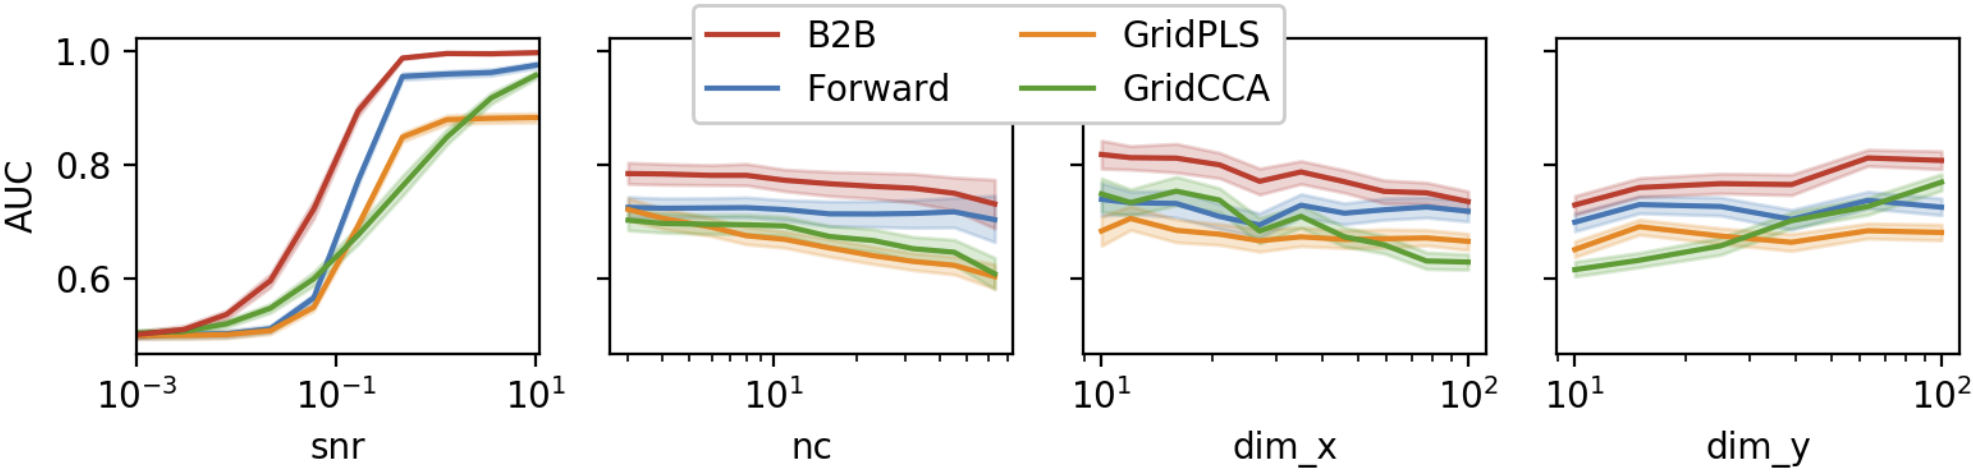
\includegraphics[width=\linewidth]{figures/AUC_conditions}
  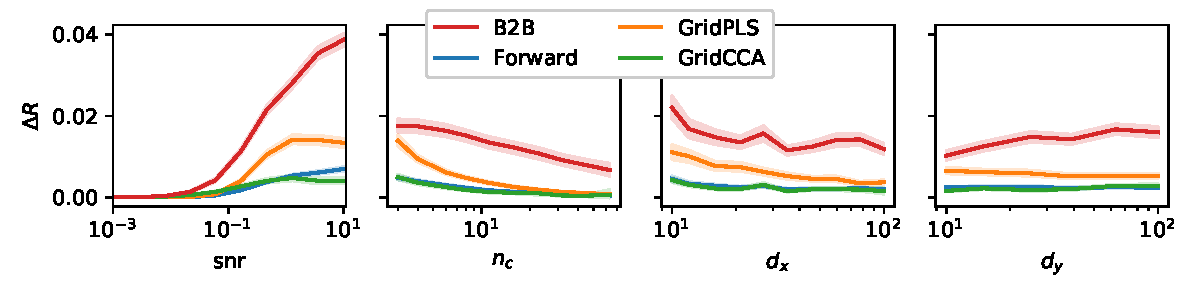
\includegraphics[width=\linewidth]{figures/R_conditions}
  \vspace{-4ex}
  \caption{Synthetic experiments. Average AUC (top) and Feature Importance $\Delta R$ (bottom) when varying experimental conditions individually. Higher is better. B2B compares favorably in all cases. \label{fig:percondition}}
\end{figure}


\subsection{Evaluating Causal Discovery with held-out prediction reliability}

In most cases, $E$ is not known and AUC can thus not be estimated.

To address this issue, we assess the ability of each model to reliably predict
independent and identically distributed data from $Y$, given all of the $X$
features versus all-but-ones feature $X_{-i}$ (i.e. 'knock-out X'). This procedure
results in two correlation metrics $R_{full}$ and $R_{knockout}$, whose
difference $\Delta R_i = R_{full}-R_{knockout}$ indicates how much each $X_i$
improves the prediction of $Y$.
%beyond what can be predicted from all other features $X_{-i}$.
In our figures, $\Delta R$ is the average of $\Delta R_i$. A higher score means that for prediction, the model relies on individual features rather than combinations of features.

We show in Appendix~\ref{appendix:feature_importance} pseudo-code to assess feature importance for our algorithm as well as baselines. For the Backward Model, feature importance cannot be assessed as there is no prediction.

% Feature importance can be computed similarly for the CCA, PLS and Forward baselines (see Appendix \ref{appendix:feature_importance}). For the Backward Model, feature importance cannot be assessed as there is no prediction.

We show in Figures~\ref{fig:percondition} (bottom) and \ref{fig:auc_plots} (right, in Appendix) that our method compares favorably to baselines.

%
% \iffalse
% For CCA and PLS, feature importance is assessed as follow:
% \begin{enumerate}
%   \item Fit $H$ and $G$ given $X_{train}$ and $Y_{train}$
%   \item For each feature $i$:
%   \begin{itemize}
%     \item Define $K$, and identity matrix whose row $i$ has been zeroed-out
%     \item Fit $H^i_k$ and $G_k$ given $X_{train} K$ and $Y_{train}$
%   \end{itemize}
% \end{enumerate}
% \fi
% For the Backward Model, feature importance cannot be assessed because there is no prediction.
% We thus simply
% report the model performance $R_i = corr(YG_i, X_i)$.


% \iffalse
% \begin{enumerate}
%
%   \item Fit $G$ given $X_{train}$ and $Y_{train}$
%   \item Fit $H$ given $X_{train}$ and $Y_{train} G^T$
%   \item For each feature $i$:
%   \begin{itemize}
%     \item Define $K$, and identity matrix whose row $i$ has been zeroed-out
%     \item Fit $H^i_k$ given $X_{train} K$ and $Y_{train} G^T$
%   \end{itemize}
%
%   \item Compute $R_{full}$ given $Y_{test} G^T$ and $X_{test}$
%   \item For all $i \in d_x$:
%   \begin{itemize}
%     \item Compute $R^i_{knockout}$ given $Y_{test} G^T$ and $X_{test} K {H^i_k}^T$
%     \item Compute $R^i_{delta}=R_{full} - R^i_{knockout}$
%   \end{itemize}
%   \end{enumerate}
% \fi

% \iffalse Ridge regression \citep{hoerl1959optimum}, multitask Lasso
% \citep{argyriou2008convex}, Partial Least Squares or PLS \citep{wold_pls,
% tenenhaus_pls}, Canonical Correlation Analysis or CCA \citep{cca_hotelling}, and
% Reduced Rank Regression or RRR \citep{Izenman_rrr}.
% %
% Each of these methods estimates a matrix of coefficients $\hat{W} \in
% \mathbb{R}^{d_x \times d_y}$, from which we estimate the diagonal mask $\hat{E}$
% using the feature importances $\hat{E}_{i,i} = \| W_{i, :} \|$.
% %
% For B2B, we obtain $\hat{E}$ as described in Algorithm~\ref{algorithm:b2br}.
% %
%
%
% We evaluate seven metrics:
% %
% test error in-distribution, test error out-distribution, test error-in
% distribution after weighting with $\hat{E}$, test error out-distribution after
% weighting with $\hat{E}$, Sonquist-Morgan false positives on $\hat{E}$,
% Sonquist-Morgan false negatives on $\hat{E}$, and the area under the ROC curve
% (AUC) between $\hat{E}$ and $E$.
% %
% The ``in-distribution'' metrics measure the test error of each predictor before
% and after weighting their features by the estimated (continuous!) mask
% $\hat{E}$.
% %
% The ``out-distribution'' metrics are similar, measuring the test error at
% samples drawn using two different random covariance matrices for both $X$ and
% $N$.
% %
% The false positives, false negatives, and AUC statistics measure the quality of
% identification of causal factors between $\hat{E}$ and the true, binary $E$.
%
% \begin{figure}[htpb] \centering
% 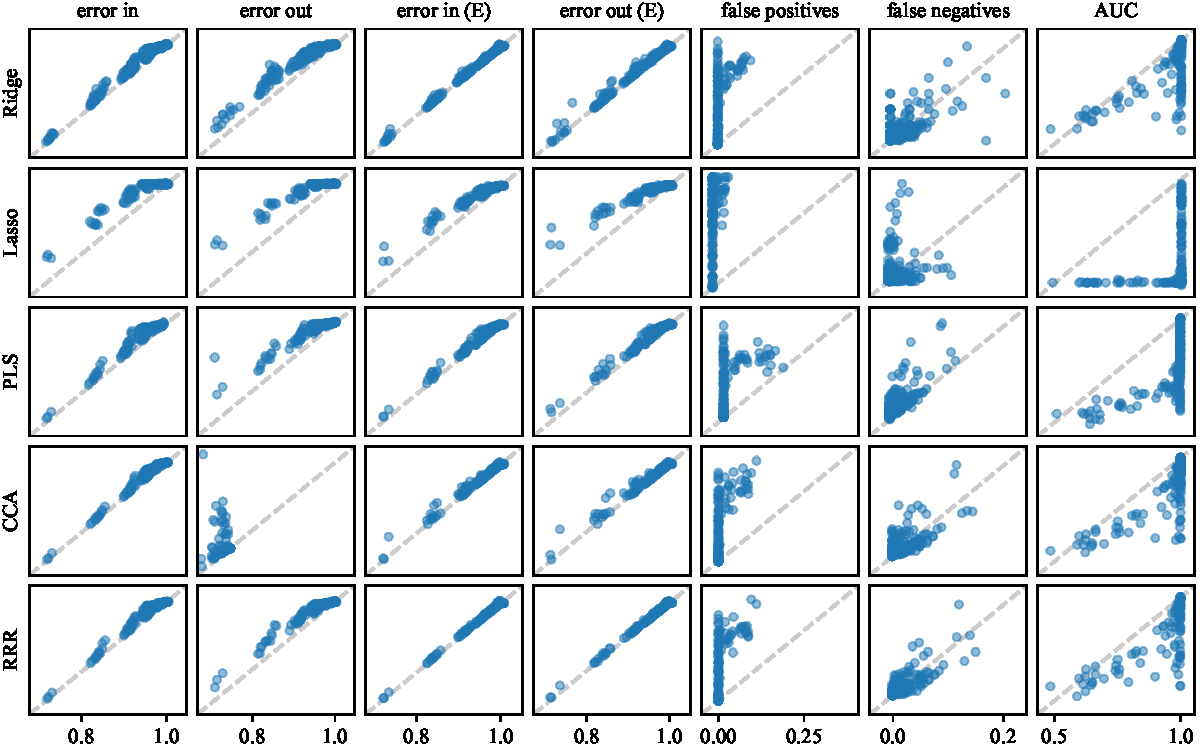
\includegraphics[width=\textwidth]{synthetic.pdf} \caption{Results of synthetic
% experiments. Each dot depicts the average value of a metric for B2B ($x$-axis)
% against a competitor ($y$-axis) for each experiment configuration averaged over
% $20$ random seeds. The prediction error on $Y$ within (in) and outside (out) of
% the training distribution are weakly but consistently larger for all of the
% models as compared to B2B with and without the Sonquist binarization (E). The
% AUC, measuring the ability of each model to separate causal from noncausal
% factors, is consistently larger in B2B as compared to the other models.}
% \label{table:synthetic} \end{figure} \fi

% Figure~\ref{table:synthetic} summarizes the results for all experimental
% conditions, metrics, and methods.
% %
% B2B is the method obtaining best test errors, lowest false positive and false
% negative discovery about $E$, and overall the best AUC when it comes to
% detecting causal influences.
